\documentclass{rvcepaper}
\begin{document}

%%%%%%%%%%%%%%%%%%%%%%%%%%%% MATHEMATICS
% ---------- MA231TB Test - 1, 9.10.2026
\begin{xpaper}
\paperinfo{deptline={Department of Mathematics}}
\par\vspace{2pt}\centerline{\bfseries\fontsize{14}{17}\selectfont Department of Mathematics}\par\vspace{6pt}
\noindent\begingroup\renewcommand{\arraystretch}{1.55}\bfseries\fontsize{11}{13}\selectfont\setlength{\tabcolsep}{4pt}
\begin{tabular}{|p{5.15cm}|C{6.05cm}|p{5.05cm}|}\hline
Date: 9.10.2026 & Test -- 1 & Max. Marks: 50\\\hline
\begin{tabular}[t]{@{}l@{}}Time: 9:30AM--11:00AM\\[4pt]Semester: III\end{tabular} &
\begin{tabular}[t]{@{}c@{}}Third Semester 2026--2027\\[4pt]Branch: AS, BT, IEM, ME\end{tabular} &
Duration: 90 minutes\\\hline
\multicolumn{2}{|p{11.45cm}|}{Course Title: STATISTICS, LAPLACE TRANSFORM AND NUMERICAL METHODS} & Course code: MA231TB\\\hline
\end{tabular}\endgroup\par\vspace{4pt}
\begin{center}\itshape
Instructions to candidates: 1. Answer all questions.\\
2. Second year mathematics hand book is allowed.
\end{center}\vspace{2pt}
\begin{xtable}{Part-A}
\q{1}{The following frequency distribution gives the enzyme concentration ($x$) and the corresponding number of fermentation batches ($f$) producing each enzyme concentration. Use the data to study the distribution of enzyme concentration by calculating the first four moments about the mean. Also evaluate $\beta_1$, $\beta_2$ and comment upon the skewness and kurtosis of the distribution.
\qtabc{|c|*{8}{c|}}{\hline $x$ & 20 & 25 & 30 & 35 & 40 & 45 & 50 & 55\\\hline $f$ & 2 & 5 & 7 & 9 & 8 & 5 & 3 & 1\\\hline}}{10}{3}{3}
\q{2a}{The following are the marks in Statistics ($x$) and the marks in Mathematics ($y$) of 10 students in I BCA examinations. Find the coefficient of rank correlation.
{\footnotesize\setlength{\tabcolsep}{3pt}\qtabc{|c|*{10}{c|}}{\hline $x$ & 43 & 96 & 74 & 38 & 35 & 43 & 22 & 56 & 35 & 80\\\hline $y$ & 30 & 94 & 84 & 38 & 30 & 18 & 30 & 41 & 48 & 95\\\hline}}}{6}{2}{2}
\q{2b}{Using the method of least squares, fit a linear relation of the form $P = a + bW$ for the following data where $P$ is the pull required to lift a weight $W$:
\qtabc{|l|c|c|c|c|}{\hline $W$(kg) & 50 & 70 & 100 & 120\\\hline $P$(kg) & 12 & 15 & 21 & 25\\\hline}}{4}{2}{3}
\q{3}{The height ($x$ cms) and weight ($y$ kgs) of 6 students are as follows. Obtain the two regression equations. Also, find the expected height of a person whose weight is 65 kgs.
\qtabc{|c|*{6}{c|}}{\hline $x$ & 153 & 157 & 168 & 160 & 170 & 163\\\hline $y$ & 48 & 50 & 50 & 49 & 54 & 53\\\hline}}{10}{2}{2}
\q{4}{Estimate $y$ at $x_1 = 10$ and $x_2 = 6$ by fitting a regression plane connecting $x_1$, $x_2$ and $y$ to the following data:
\qtabc{|c|*{6}{c|}}{\hline $y$ & 90 & 72 & 54 & 42 & 30 & 12\\\hline $x_1$ & 3 & 5 & 6 & 8 & 12 & 14\\\hline $x_2$ & 16 & 10 & 7 & 4 & 3 & 2\\\hline}}{10}{3}{2}
\q{5}{Determine the value of $u(x,y)$ satisfying the Laplace equation $\dfrac{\partial^2 u}{\partial x^2} + \dfrac{\partial^2 u}{\partial y^2} = 0$ at the pivotal points of a square region with boundary values as shown in the figure. Carry out 5 iterations.
\par\vspace{3pt}\centerline{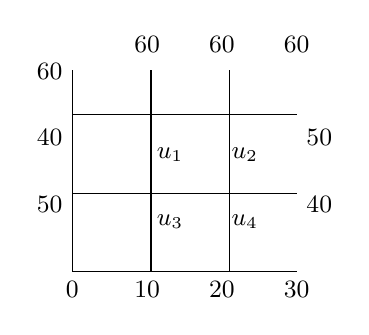
\begin{tikzpicture}[x=0.95cm,y=0.85cm,font=\small,line cap=rect]
 \draw (0,0) grid (3,3);
 \node[below right] at (1,2) {$u_1$}; \node[below right] at (2,2) {$u_2$};
 \node[below right] at (1,1) {$u_3$}; \node[below right] at (2,1) {$u_4$};
 \node[above=3pt] at (1,3) {60}; \node[above=3pt] at (2,3) {60}; \node[above=3pt] at (3,3) {60};
 \node[left] at (0,3) {60}; \node[left] at (0,2) {40}; \node[left] at (0,1) {50};
 \node[right] at (3,2) {50}; \node[right] at (3,1) {40};
 \node[below] at (0,0) {0}; \node[below] at (1,0) {10}; \node[below] at (2,0) {20}; \node[below] at (3,0) {30};
\end{tikzpicture}}\par}{10}{3}{3}
\end{xtable}
\btfoot{|l|l|*{10}{C{0.85cm}|}}{\hline
\multirow{2}{*}{Marks Distributions} & Particulars & CO1 & CO2 & CO3 & CO4 & L1 & L2 & L3 & L4 & L5 & L6\\\cline{2-12}
& Max Marks & -- & 26 & 24 & -- & -- & 20 & 30 & -- & -- & --\\\hline}
\end{xpaper}

% ---------- MA231TB CIE - I, 21.10.2024
\begin{xpaper}
\paperinfo{deptline={Department of Mathematics},date={21.10.2024},exam={Quiz -- I \& Test -- I},maxmarks={10 + 50},sem={III},prog={AS, BT, CH, ME, IEM},duration={9.30 AM -- 11.30 AM},
 title={Statistics, Laplace Transform and Numerical Methods},code={MA231TB}}
\xhead
\begin{xtable}{Questions}
\qpart{Part -- A}
\q{1}{For a statistical data with n = 5, $\sum x$ = 18, $\sum y$ = 15, $\sum x^2$ = 110 and $\sum xy$ = 71, the best fit straight line by the method of least squares is \blank[2.2cm].}{1}{1}{1}
\q{2}{For a distribution the mean is 12 and the variance is 19. Then the second moment about the mean is \blank[1.8cm].}{1}{1}{2}
\q{3}{The first two moments about the point x = 2 are 1 and 16, then the second central moment is \blank[1.8cm].}{2}{2}{2}
\q{4}{The equations of regression lines are y = 0.5x + p and y = 0.4y + q, then the correlation coefficient is \blank[1.8cm].}{2}{2}{2}
\q{5}{$\mathcal{L}[\sin 3t + \cosh 5t]$ = \blank[1.8cm].}{1}{1}{1}
\q{6}{$\mathcal{L}[(t^2e^{3t})]$ = \blank[1.8cm].}{1}{1}{2}
\q{7}{$\mathcal{L}[(e^{-5t} + e^t)^2]$ = \blank[1.8cm].}{2}{2}{1}
\qpart{Part -- B}
\q{1}{Determine the equation of the regression plane connecting $x_1$, $x_2$ and y, given
\qtabc{|l|c|c|c|c|c|c|}{\hline Diffusion time (hours) $x_1$ & 1.5 & 2.5 & 0.5 & 1.2 & 2.6 & 0.3\\\hline Sheet-resistance (Ohms-cm) $x_2$ & 66 & 87 & 69 & 141 & 93 & 105\\\hline Current gain (y) & 5.3 & 7.8 & 7.4 & 9.3 & 10.8 & 9.1\\\hline}
Estimate y at $x_1$ = 1.8 and $x_2$ = 112.}{10}{--}{4}
\q{2}{The marks obtained by 50 students in a Mathematics test are given below:
\qtabc{|l|c|c|c|c|c|c|}{\hline Marks & 10--20 & 20--30 & 30--40 & 40--50 & 50--60 & 60--70\\\hline No. of students & 4 & 8 & 10 & 15 & 8 & 5\\\hline}
Compute first four moments about the mean and also find the measures $\beta_1$ and $\beta_2$ for the following distribution and comment on the nature of distribution of students.}{10}{--}{3}
\q{3a}{The following pairs of observations were noted in an experimental work on cosmic rays. Find by the method of least squares the most possible values of a and b for the equation y = a + bx which fits the data.
\qtabc{|l|c|c|c|c|c|c|}{\hline x & 1 & 2 & 3 & 4 & 5 & 6\\\hline y & 2.98 & 4.26 & 5.21 & 6.10 & 6.80 & 7.50\\\hline}
Predict y when x = 3.75.}{6}{--}{1}
\q{3b}{The coefficient of rank correlation obtained by ten students in statistics and accountancy was 0.2. It was later discovered that the difference in ranks in the two subjects of one of the students was wrongly taken as 9 instead of 7. Find the correct rank correlation coefficient.}{4}{--}{2}
\q{4}{A study was made on the amount of converted sugar in a certain process at various temperatures. The data were coded and recorded as follows:
\qtabc{|l|*{10}{c|}}{\hline x & 1.1 & 1.2 & 1.3 & 1.4 & 1.5 & 1.6 & 1.7 & 1.8 & 1.9 & 2.0\\\hline y & 7.8 & 8.5 & 9.8 & 9.5 & 8.9 & 8.6 & 10.2 & 9.3 & 9.2 & 10.5\\\hline}
Construct the table of values and compute the correlation coefficient for this data and also find the regression lines of x on y and y on x.}{10}{--}{3}
\q{5}{Determine the transformation in frequency domain if the signal in time domain is given by $f(t) = \dfrac{\cos 6t - \cos 3t}{t} + e^{-5t}\sin 2t\cos 3t + t(\sqrt{t}+1)^2$.}{10}{--}{2}
\end{xtable}
\end{xpaper}

%%%%%%%%%%%%%%%%%%%%%%%%%%%% WORK SYSTEMS DESIGN
% ---------- IM233AI CIE - I, 14th Oct 2026
\begin{iempaper}
\paperinfo{dept={INDUSTRIAL ENGINEERING \& MANAGEMENT},date={14\textsuperscript{th} Oct 2026},exam={CIE -- I},maxmarks={50},sem={III},prog={UG},duration={90 Min},
 title={WORK SYSTEMS DESIGN},code={IM233AI}}
\iemhead
\begin{cietable}{M}{BT}{CO}
\q{1}{Describe the elements of a worker-machine system. How does it differ from a fully automated system?}{10}{3}{CO1}
\q{2}{A work group of 5 workers in a certain month produced 500 units of output working 8 hr/day for 22 days in the month. (a) What productivity measures could be used for this situation, and what are the values of their respective productivity ratios? (b) Suppose that in the next month, the same work group produced 600 units but there were only 20 workdays in the month. Using the same productivity measures as before, determine the productivity index using the prior month as a base.}{10}{3}{CO1}
\q{3}{Analyse the three categories of excess non-productive activities generally carried out in organizations.}{10}{3}{CO2}
\q{4}{Enumerate the steps involved in conducting a Method Study by an Industrial Engineer in organizations.}{10}{2}{CO2}
\q{5}{How does traditional IE charting techniques aid in identifying non-value-added elements/motions of work. Provide two examples.}{10}{2}{CO2}
\end{cietable}
\end{iempaper}

% ---------- IM233AI CIE - I, 21st October 2024
\begin{iempaper}
\paperinfo{dept={INDUSTRIAL ENGINEERING \& MANAGEMENT},date={21\textsuperscript{st} October 2024},exam={CIE -- I},maxmarks={10 + 50},sem={III},prog={UG},duration={120 Min},
 title={WORK SYSTEMS DESIGN},code={IM233AI}}
\iemhead
\begin{cietable}{M}{BT}{CO}
\qpart{Part -- A}
\q{1}{What is meant by the term Work?}{02}{2}{1}
\q{2}{Illustrate the Pyramidal Structure of the task.}{02}{3}{1}
\q{3}{Distinguish between methods design and methods engineering.}{02}{2}{2}
\q{4}{Mention the elements of Standard Time.}{02}{2}{1}
\q{5}{What are the two common measures used in industry to assess a worker's productivity?}{02}{1}{1}
\qpart{Part -- B}
\q{1}{Distinguish between Production and Productivity. Explain with suitable illustrations on the ways and means to enhance productivity in organizations.}{10}{3}{1}
\q{2}{A work group of 10 workers in a certain month produced 1000 units of output working 8 hr/day for 22 days in the month. What productivity measures could be used for this situation? Suppose that in the next month, the same work group produced 1200 units but there were only 20 work days in the month. Using the same productivity measures as before, determine the productivity index using the prior month as a base.}{10}{3}{1}
\q{3}{The normal time to perform a repetitive manual task is 3.25 minutes. In addition, an irregular work element whose normal time is 1.5 minutes must be performed every 8 cycles. Two work units are produced each cycle. The PFD allowance is 12\%. Determine the standard time per piece. How many work units are produced in an 8 hour shift at standard performance? Determine the anticipated amount of time worked and the amount of time lost per 8 hour shift that corresponds to the PFD allowance factor of 14\%.}{10}{3}{3}
\q{4}{Enumerate the steps involved in conducting a Method Study by an Industrial Engineer in organizations.}{10}{2}{2}
\q{5a}{Classify the worker-machine systems according to number of machines and workers.}{05}{1}{1}
\q{5b}{What does PFD stand for? Bring out the purpose of PFD allowance in determining the standard time for a task.}{05}{3}{1}
\end{cietable}
\end{iempaper}

% ---------- IM233AI CIE - I, 9th January 2024
\begin{iempaper}
\paperinfo{dept={INDUSTRIAL ENGINEERING \& MANAGEMENT},date={9\textsuperscript{th} January 2024},exam={CIE -- I},maxmarks={50},sem={III},prog={UG},duration={90 Min},
 title={WORK SYSTEMS DESIGN},code={IM233AI}}
\iemhead
\begin{cietable}{M}{BT}{CO}
\q{1}{Analyze the three categories of excess non-productive activities generally carried out in organizations.}{10}{4}{1}
\q{2}{A work group of 10 workers in a certain month produced 7200 units of output working 8 hours per day for 22 days in the month. Determine the labor productivity ratio using units of output per worker hour and units of output per worker month. Suppose that in the next month, the same work group produced 6800 units but there were only 20 workdays in the month. For each productivity measure, determine the productivity index for the next month using prior month as a base.}{10}{3}{1}
\q{3}{The normal time to perform a certain manual work cycle is 3.47 minutes. In addition, an irregular work element whose normal time is 3.70 minutes must be performed every 10 cycles. One work unit is produced each cycle. The PFD allowance factor is 14\%. Determine the standard time per piece and how many work units are produced during an 8 hour shift at 100 percent performance and the worker works exactly 7.018 hours, which corresponds to 14 percent allowance factor. If the worker's performance is 120 percent and works 7.2 hours during regular shift, how many units are produced?}{10}{3}{3}
\q{4}{Distinguish between Production and Productivity. Also justify the rationale for considering labor productivity as a measure of organizational efficiency and effectiveness.}{10}{3}{1}
\q{5a}{Enumerate any five reasons for variations in work cycle times in manual work systems.}{05}{2}{1}
\q{5b}{Illustrate the classification of powered machinery in worker machine system.}{05}{3}{1}
\end{cietable}
\end{iempaper}

% ---------- 21IM33 CIE - I, 18th January 2023
\begin{iempaper}
\paperinfo{dept={INDUSTRIAL ENGINEERING \& MANAGEMENT},date={18\textsuperscript{th} January 2023},exam={CIE -- I},maxmarks={10 + 50},sem={III},prog={UG},duration={20 + 90 Min},
 title={WORK SYSTEMS DESIGN},code={21IM33}}
\iemhead
\begin{cietable}{M}{BT}{CO}
\qpart{Part -- A}
\q{1}{What is meant by the term Work?}{02}{2}{1}
\q{2}{Illustrate the Pyramidal Structure of the task.}{02}{3}{1}
\q{3}{How is Motion Study different from methods engineering?}{02}{2}{2}
\q{4}{What is meant by productivity?}{02}{2}{1}
\q{5}{List the three categories of principles of motion economy.}{02}{1}{2}
\qpart{Part -- B}
\q{1}{Analyze the problems encountered by organizations in measuring productivity.}{10}{4}{1}
\q{2}{A work group of 5 workers in a certain month produced 500 units of output working 8 hr/day for 22 days in the month. What productivity measures could be used for this situation? Suppose that in the next month, the same work group produced 600 units but there were only 20 work days in the month. Using the same productivity measures as before, determine the productivity index using the prior month as a base.}{10}{3}{1}
\q{3}{Enumerate the principles of motion economy related to the use of Human body.}{10}{2}{2}
\q{4}{Methods engineering can be categorized into Methods analysis and Methods design. Distinguish between them in terms of their scope, objectives and applications.}{10}{3}{2}
\q{5}{The normal time to perform a repetitive manual task is 4.25 minutes. In addition, an irregular work element whose normal time is 1.75 minutes must be performed every 8 cycles. Two work units are produced each cycle. The PFD allowance is 16\%. Determine the standard time per piece. How many work units are produced in an 8 hour shift at standard performance? Determine the anticipated amount of time worked and the amount of time lost per 8 hour shift that corresponds to the PFD allowance factor of 16\%.}{10}{3}{3}
\end{cietable}
\end{iempaper}

% ---------- 18IM35 CIE - I, September 2019
\begin{xpaper}
\paperinfo{deptline={Department of Industrial Engineering and Management},date={September 2019},exam={CIE -- I},maxmarks={50},sem={III},prog={UG},duration={90 Min},
 title={Work Systems Design},code={18IM35}}
\xhead
\begin{xtable}{Questions (Part -- B)}
\q{1a}{Distinguish between Labour productivity ratio and Labour Productivity Index.}{05}{2}{1}
\q{1b}{Distinguish between work system as a physical entity and work system as a profession.}{05}{2}{1}
\q{2}{A work group of 5 workers in a certain month produced 500 units of output working 8 hr/day for 22 days. (i) What productivity measures could be used for this situation, and what are the values of their respective productivity ratios? (ii) Suppose that in the next month, the same work group produced 600 units but there were only 20 work days in the month. Using the same productivity measures as before, determine the productivity index using the prior month as a base.}{10}{3}{1}
\q{3}{The normal time to perform a certain manual work cycle is 3.47 min. In addition, an irregular work element whose normal time is 3.70 min must be performed every 10 cycles. One work unit is produced each cycle. The PFD allowance factor is 14\%. Determine (i) the standard time per piece and (ii) how many work units are produced during an 8-hour shift at 100\% performance, and the worker works exactly 7.018 hr, which corresponds to the 14\% allowance factor. (iii) If the worker's pace is 120\% and he works 7.2 hours during the regular shift, how many units are produced?}{10}{4}{3}
\q{4}{Distinguish between the following along with an example for each. (i) Office automation vs. Office augmentation (ii) Office activities vs. Office applications.}{10}{2}{1}
\q{5}{Review any five principles related to the design of tooling and equipment.}{10}{4}{2}
\end{xtable}
\end{xpaper}

%%%%%%%%%%%%%%%%%%%%%%%%%%%% MANUFACTURING PROCESSES
% ---------- IM334AI CIE - I, 14th Oct 2026
\begin{iempaper}
\paperinfo{dept={INDUSTRIAL ENGINEERING \& MANAGEMENT},date={14\textsuperscript{th} Oct 2026},exam={CIE -- I},maxmarks={50},sem={III},prog={UG},duration={90 Min},
 title={MANUFACTURING PROCESS \& AUTOMATION},code={IM334AI}}
\begingroup\patchcmd{\iemhead}{Course Title: \getkey{title}}{\raggedright Course Title: \getkey{title}}{}{}\iemhead\endgroup
\begin{cietable}{M}{BT}{CO}
\q{1}{Explain the procedure for making a sand mould and discuss the important aspects of mould preparation.}{10}{1}{1}
\q{2}{Explain the important properties of moulding sand and discuss their significance in producing defect-free castings.}{10}{1}{2}
\q{3}{A company wants to manufacture long aluminium sections with a constant and complex cross-section for building and automotive applications.
\begin{abc}\item Select a suitable manufacturing process.\item Explain its principle with sketch.\end{abc}}{10}{3}{4}
\q{4}{A carbide cutting tool used for machining a high-temperature alloy develops a large depression on the rake face after prolonged operation.
\begin{abc}\item Identify the type of wear.\item Explain how it develops.\item What are its effects?\item How can it be controlled?\end{abc}}{10}{3}{3}
\q{5}{A machining operation currently runs at 150 m/min and has a tool life of 40 minutes. The production engineer wants to increase cutting speed to 200 m/min. Assume Taylor's exponent ($n = 0.25$). Determine the new tool life.}{10}{3}{2}
\end{cietable}
\end{iempaper}

% ---------- IM234AI CIE - I, 22nd October 2024
\begin{iempaper}
\paperinfo{dept={INDUSTRIAL ENGINEERING \& MANAGEMENT},date={22\textsuperscript{nd} October 2024},exam={CIE -- I},maxmarks={10 + 50},sem={III},prog={UG},duration={120 Min},
 title={MANUFACTURING PROCESSES},code={IM234AI}}
\iemhead
\begin{cietable}{M}{BT}{CO}
\qpart{Part -- A}
\q{1}{\blank[1.8cm] is the passage through which the molten metal from pouring basin reaches the mould cavity.}{1}{L1}{CO1}
\q{2}{\blank[1.8cm] colour on surface of pattern is used to indicate the product has to be finished.}{1}{L2}{CO1}
\q{3}{Balanced core is also called a \blank[1.8cm] core.}{1}{L2}{CO2}
\q{4}{Loam sand is a mixture of \blank[1.8cm].}{1}{L1}{CO2}
\q{5}{\blank[1.8cm] Pattern is used for generating axi-symmetrical and prismatic shapes.}{1}{L2}{CO3}
\q{6}{Coining is the operation of \blank[1.8cm] forging.}{1}{L1}{CO2}
\q{7}{List different types of moulding sand.}{2}{L1}{CO3}
\q{8}{Why chaplets are used in moulding process?}{2}{L2}{CO2}
\qpart{Part -- B}
\q{1}{The foundry uses silica sand, mixed with bentonite clay as a binder, to create moulds for casting aluminum components. For a critical part, a complex valve body for an engine, the production has resulted in a high rejection rate due to defects. Your role is to conduct a case study based on a detailed analysis of the sand mould making procedure, assess the possible causes of these defects.}{10}{L2}{CO1}
\q{2}{Explain the process used for pushing the billet or slug of metal through a die orifice, thus forming an elongated part of uniform cross section corresponding to the shape of the die?}{10}{L2}{CO3}
\q{3}{The foundry has been manufacturing engine components using sand casting. During quality checks, several castings were found to be either slightly undersized or oversized compared to the required dimensions. The investigation suggests that the allowances applied to the pattern might not be correctly calculated or uniformly applied. You have been tasked with reviewing the process and making recommendations to improve accuracy.}{10}{L3}{CO2}
\q{4}{``Jolt and squeeze moulding machine is used for preparing the moulds at faster rate and with high quality''. Explain with a neat sketch.}{10}{L1}{CO2}
\q{5}{Explain the working principle of Hydro-forming Process with its limitations.}{10}{L2}{CO1}
\end{cietable}
\end{iempaper}

% ---------- IM234AI CIE - I, 9th January 2024
\begin{iempaper}
\paperinfo{dept={INDUSTRIAL ENGINEERING \& MANAGEMENT},date={9\textsuperscript{th} January 2024},exam={CIE -- I},maxmarks={50},sem={III},prog={UG},duration={90 Min},
 title={MANUFACTURING PROCESS},code={IM234AI}}
\iemhead
\begin{cietable}{M}{BT}{CO}
\q{1}{Discuss the objectives expected to be achieved through efficient and economical machining?}{10}{1}{1}
\q{2}{Draw a neat sketch of a single point cutting tool indicating its complete geometry.}{10}{2}{2}
\q{3}{How many types of chips are formed in metal cutting? List the factors that are responsible for formation of these chips.}{10}{3}{3}
\q{4}{Explain crater wear and flank wear of a tool with a neat sketch.}{10}{2}{2}
\q{5}{In orthogonal cutting of a work piece, the following data were obtained: Feed force = 350 kgf, Cutting force = 150 kgf, Chip thickness ratio = 0.44, Rake angle = 10$^{\circ}$. Calculate the shear angle, shear force and normal force.}{10}{2}{3}
\end{cietable}
\end{iempaper}

% ---------- 21IM34 CIE - I, 19th January 2023
\begin{iempaper}
\paperinfo{dept={INDUSTRIAL ENGINEERING AND MANAGEMENT},date={19\textsuperscript{th} January 2023},exam={CIE -- I},maxmarks={10 + 50},sem={III},prog={UG},duration={20 + 90 Min},
 title={MANUFACTURING PROCESS},code={21IM34}}
\iemhead
\begin{cietable}{M}{BT}{CO}
\qpart{Part -- A}
\q{1.1}{In \blank[1.8cm] forging operation, repeated hammering and closed die is used.}{01}{L2}{CO1}
\q{1.2}{\blank[1.8cm] Molding machine gives better packing of sand near pattern.}{01}{L1}{CO2}
\q{1.3}{In sand molding, the bottom most part of the flask is called \blank[1.8cm].}{01}{L2}{CO1}
\q{1.4}{Over hang core is also called as \blank[1.8cm].}{01}{L1}{CO2}
\q{1.5}{\blank[1.8cm] Pattern are generally used for circular castings.}{01}{L2}{CO1}
\q{1.6}{Irregular depressions on the surface of the forging is the \blank[1.8cm] defect in forging.}{01}{L3}{CO2}
\q{1.7}{Define porosity?}{02}{L1}{CO1}
\q{1.8}{List any two limitations of Extrusion process.}{02}{L2}{CO2}
\qpart{Part -- B}
\q{1}{Define pattern? List the types of patterns and explain any two briefly.}{10}{L2}{CO2}
\q{2}{``Sand slinger moulding machine is used for preparing the moulds at faster rate and with high quality''. Explain with a neat sketch.}{10}{L2}{CO1}
\q{3}{``Molding processes to produce internal cavities and reentrant angles''. What is the process called and explain the different types.}{10}{L3}{CO2}
\q{4}{Explain the stages in drop forging a connecting rod for an internal combustion engine.}{10}{L3}{CO1}
\q{5}{Briefly explain the principle of Rolling with a neat sketch.}{10}{L3}{CO1}
\end{cietable}
\end{iempaper}

% ---------- 18IM36 CIE - I, September 2019
\begin{xpaper}
\paperinfo{deptline={Department of Industrial Engineering and Management},date={September 2019},exam={CIE -- I},maxmarks={50},sem={III},prog={UG},duration={90 Min},
 title={Manufacturing Process},code={18IM36}}
\xhead
\begin{xtable}{Questions (Part -- B)}
\q{1}{Discuss orthogonal \& oblique cutting with respect to the following: (i) Angle of contact (ii) Depth of cut (iii) Chip form (iv) Area of contact.}{10}{2}{2}
\q{2}{State the assumptions made by Merchant while constructing a Merchant Circle diagram.}{10}{2}{2}
\q{3}{In an orthogonal turning operation on a lathe the following data were obtained: Cutting force = 120 kg, Feed force = 30 kg, Back rake angle = 15$^{\circ}$, Feed rate = 0.2 mm/rev, chip thickness = 0.3 mm, Cutting speed = 100 m/min, Work piece diameter = 120 mm, depth of cut = 0.4 mm. Calculate chip thickness ratio, shear angle, coefficient of friction, friction angle, shear stress, shear strain, strain energy and chip flow velocity.}{10}{1}{1}
\q{4}{In a tool wear test with a high speed steel cutting tool, the following values of tool life were obtained:
\qtabc{|c|c|}{\hline Tool Life & Cutting Speed\\\hline 30 min & 25.0 m/min\\\hline 1.5 min & 70.0 m/min\\\hline}
Calculate the values of `n' \& `c' using Taylor's Tool Life equation.}{10}{1}{1}
\q{5}{Discuss the factors which affect the parameters of Tool Life.}{10}{2}{2}
\end{xtable}
\end{xpaper}

%%%%%%%%%%%%%%%%%%%%%%%%%%%% DIGITAL METROLOGY
% ---------- IM335AI CIE - I, 13th Oct 2026
\begin{iempaper}
\paperinfo{dept={INDUSTRIAL ENGINEERING \& MANAGEMENT},date={13\textsuperscript{th} Oct 2026},exam={CIE -- I},maxmarks={50},sem={III},prog={UG},duration={90 Min},
 title={Digital Measurements and Metrology},code={IM335AI}}
\iemhead
\begin{cietable}{M}{BT}{CO}
\q{1}{Describe the three stages of a generalized measurement system with a neat block diagram. Illustrate the application of these stages in pressure measurement using a Bourdon-tube pressure gauge.}{10}{L3}{CO1}
\q{2}{List different static characteristics of measuring instruments. Explain each characteristic with suitable sketches or response curves wherever applicable, and discuss their importance in achieving effective measurement system performance.}{10}{L2}{CO1}
\q{3}{Explain the principle, construction, and working of a capacitive transducer with a neat sketch. Discuss the different methods of varying capacitance, along with its advantages, limitations, and applications.}{10}{L3}{CO1}
\q{4}{Describe the principle, construction, and working of a Hall Effect sensor with a neat sketch. Explain the generation of Hall voltage when a magnetic field is applied to a current-carrying conductor or semiconductor, and state its important applications.}{10}{L3}{CO1}
\q{5}{Illustrate the principle, construction, and working of a potentiometer-type displacement sensor with a neat sketch. Discuss the use of linear and rotary potentiometers for position and displacement measurement, along with their advantages and limitations.}{10}{L3}{CO1}
\end{cietable}
\end{iempaper}

% ---------- IM235AI CIE - I, 23rd October 2024
\begin{iempaper}
\paperinfo{dept={INDUSTRIAL ENGINEERING \& MANAGEMENT},date={23\textsuperscript{rd} October 2024},exam={CIE -- I},maxmarks={10 + 50},sem={III},prog={UG},duration={150 Min},
 title={DIGITAL METROLOGY},code={IM235AI}}
\iemhead
\begin{cietable}{M}{BT}{CO}
\qpart{Part -- A}
\q{1}{The \blank[1.8cm] stage may include amplification, filtering, and conversion of signals into a format that can be further processed.}{01}{L1}{CO1}
\q{2}{The \blank[1.8cm] in the intermediate stage transfers and amplifies the mechanical movement from the Bourdon tube.}{01}{L2}{CO1}
\q{3}{For optical measuring systems, \blank[1.8cm] can be an example for Detector Transducer Stage.}{01}{L2}{CO1}
\q{4}{\blank[1.8cm] refers to the smallest change in a measured variable that an instrument can detect.}{01}{L2}{CO1}
\q{5}{\blank[1.8cm] is the extent to which a measurement system can maintain its accuracy over time without recalibration.}{01}{L1}{CO1}
\q{6}{\blank[1.8cm] is the minimum value of the input quantity to which an instrument responds and indicates a change in the output value.}{01}{L1}{CO1}
\q{7}{The difference between the actual value of a changing quantity and the measured value due to the system's response characteristics is referred to as \blank[1.8cm].}{01}{L2}{CO1}
\q{8}{In the context of optical transducer, the primary function of a \blank[1.8cm] is to sense light and convert it into a measurable electrical signal.}{01}{L2}{CO2}
\q{9}{\blank[1.8cm] involves comparing the measurement output of an instrument directly against a known standard.}{01}{L2}{CO2}
\q{10}{A \blank[1.8cm] is a type of resistive transducer that measures the deformation of an object by detecting changes in electrical resistance.}{01}{L2}{CO2}
\qpart{Part -- B}
\q{1}{Explain briefly the three stages of a generalized measurement system with block diagram. Consider any two examples and identify the three stages of measurement.}{10}{L2}{CO1}
\q{2}{Describe briefly the important static and dynamic characteristics of Measurement systems with suitable sketches and graphs. How can the integration of both static and dynamic characteristics optimize the performance of a measurement system.}{10}{L2}{CO1}
\q{3}{Describe the structure of an LVDT and explain how the movement of the core within the coils induces a voltage that is proportional to its position. Provide examples of various industrial applications where LVDT's are used for measurement.}{10}{L3}{CO2}
\q{4}{Describe the working principle and applications of eddy current proximity sensors in metrology. Evaluate the effectiveness of eddy current proximity sensors in monitoring the rotational speed of turbine blades in high-speed industrial machinery, considering challenges and optimizations for optimal performance.}{10}{L3}{CO2}
\q{5}{Explore the utilization of tachogenerators in metrology, focusing on their application in measuring rotational speed. Discuss the application of tachogenerators in providing real-time speed feedback within automated manufacturing systems.}{10}{L3}{CO2}
\end{cietable}
\end{iempaper}

% ---------- IM235AI CIE - I, 10th January 2024
\begin{iempaper}
\paperinfo{dept={INDUSTRIAL ENGINEERING \& MANAGEMENT},date={10\textsuperscript{th} January 2024},exam={CIE -- I},maxmarks={50},sem={III (2022 scheme)},prog={UG},duration={90 Min},
 title={DIGITAL METROLOGY},code={IM235AI}}
\iemhead
\begin{cietable}{M}{BT}{CO}
\q{1}{Explain briefly the three stages of a generalized measurement system with block diagram. Consider any two examples and identify the three stages of measurement.}{10}{L2}{CO1}
\q{2}{Describe briefly the important static and dynamic characteristics of Measurement systems with suitable sketches and graphs. How can the integration of both static and dynamic characteristics optimize the performance of a measurement system, and what considerations should be taken into account to ensure a balanced and effective design.}{10}{L3}{CO1}
\q{3}{Enumerate briefly on different types of Standards and Calibration. Explain the role of calibration in ensuring accuracy and reliability in measurements, and how do standards contribute to the traceability of measurements in various industries.}{10}{L3}{CO1}
\q{4}{Explain the principle of a Resistive Transducers. Explain any two Resistive Transducers with neat sketches.}{10}{L2}{CO1}
\q{5}{Discuss briefly on the statistical Evaluation of measured data. What role does statistical analysis play in assessing the accuracy and precision of measured data, provide examples of specific statistical tests commonly used for this purpose.}{10}{L2}{CO1}
\end{cietable}
\end{iempaper}

% ---------- 18IM33 CIE - I, September 2019
\begin{xpaper}
\paperinfo{deptline={Department of Industrial Engineering and Management},date={September 2019},exam={CIE -- I},maxmarks={50},sem={III},prog={UG},duration={90 Min},
 title={Metrology and Measurements},code={18IM33}}
\xhead
\begin{xtable}{Questions}
\q{Q1}{With an example, enumerate on the generalized measurement system. Justify the answer by considering bourdon tube as an example. Describe with neat sketches and block diagrams.}{10}{L2}{CO1}
\q{Q2a}{Describe briefly the different static characteristics of Measurement systems.}{06}{L2}{CO2}
\q{Q2b}{Define Error. Explain briefly the different types of Errors and remedies to resolve them.}{04}{L2}{CO2}
\q{Q3a}{Define (i) Maximum Clearance (ii) Basic Shaft (iii) Fundamental Deviation and schematically represent it.}{06}{L1}{CO1}
\q{Q3b}{Enumerate on the concept (i) Interchangeability (ii) Hole basis systems.}{04}{L2}{CO2}
\q{Q4}{Determine the tolerances on the hole and the shaft for a precision running fit designated by 25H7g6, given: 25 mm lies between 18--30 mm; Fundamental deviation for g shaft = $-$16D$^{0.44}$; IT7 = 16i and IT6 = 10i. State the actual maximum and minimum sizes of the hole and shaft and maximum and minimum clearances and represent all the dimensions graphically.}{10}{L4}{CO2}
\q{Q5a}{Define Fit. Explain briefly the various types of fits with examples.}{10}{L2}{CO2}
\end{xtable}
\end{xpaper}

%%%%%%%%%%%%%%%%%%%%%%%%%%%% HUMAN RESOURCE MANAGEMENT
% ---------- IM236AT CIE - I, 13th Oct 2026
\begin{iempaper}
\paperinfo{dept={INDUSTRIAL ENGINEERING \& MANAGEMENT},date={13\textsuperscript{th} Oct 2026},exam={CIE -- I},maxmarks={50},sem={III},prog={UG},duration={90 Min},
 title={HUMAN RESOURCE MANAGEMENT \& ANALYTICS},code={IM236AT}}
\begingroup\patchcmd{\iemhead}{Course Title: \getkey{title}}{\raggedright Course Title: \getkey{title}}{}{}\iemhead\endgroup
\begin{cietable}{M}{BT}{CO}
\q{1}{A software company is recruiting Data Analysts, but newly recruited employees are unable to meet the expectations of their managers. Apply the concept of Job Analysis to identify the possible gaps and suggest the information that should be collected about the job.}{10}{L3}{1}
\q{2}{Explain the importance of training, development and performance appraisal in improving employee and organizational performance.}{10}{L2}{3}
\q{3}{An IT company with 800 employees is revising its HR policies. Consider the following situations and select the appropriate HR policy type for each. Give a brief justification.
\begin{abc}
\item A newly established company develops its own recruitment principles based on its organizational philosophy.
\item Employees want clear rules regarding promotion, transfer and working hours.
\item An employee approaches HR seeking medical benefits during prolonged sickness.
\item Management introduces a broad policy covering employee transportation, housing support and allowances.
\item The company makes attendance at technical training compulsory at specified intervals.
\item Management documents the grievance redressal and employee participation procedure.
\end{abc}}{10}{L3}{3}
\q{4}{Discuss the evolution of HRM and its importance.}{10}{L2}{2}
\q{5}{Develop the best human resource practices that could be implemented in the start-up companies.}{10}{L3}{4}
\end{cietable}
\end{iempaper}

%%%%%%%%%%%%%%%%%%%%%%%%%%%% BASKET / OTHER-DEPARTMENT COURSES
% ---------- CV232TA Environment and Sustainability, CIE - I, 09/10/2026
\begin{xpaper}
\paperinfo{shownote=0}
\par\vspace{2pt}\centerline{\bfseries\fontsize{14}{17}\selectfont Department of Civil Engineering}\par\vspace{6pt}
\noindent\begingroup\renewcommand{\arraystretch}{1.45}\bfseries\fontsize{11}{13}\selectfont
\begin{tabular}{|p{4.2cm}|p{4.6cm}|p{4.2cm}|p{3.6cm}|}\hline
Date & 09/10/2026 & Maximum Marks & 50\\\hline
Course Code & CV232TA & Duration & 90 Min\\\hline
Sem & III & \multicolumn{2}{l|}{CIE -- I}\\\hline
\multicolumn{4}{|c|}{Environment and Sustainability (Basket Course)}\\\hline
\end{tabular}\endgroup\par\vspace{6pt}
\begin{cietable}{M}{BT}{CO}
\q{1.}{Classify different types of eco system and explain any two briefly.}{10}{2}{1}
\q{2.}{Define solid waste management and list the objectives of solid waste management.}{10}{2}{1}
\multirow{2}{*}{3.} & i) The design population of a town is 15000. Determine the average daily demand, maximum hourly demand. Assume per capita consumption as 270 LPCD, Maximum daily demand as 1.8 times average daily demand and maximum hourly demand as 2.7 times annual average hourly demand. & 05 & 3 & 1\\ \cline{2-5}
& ii) A city generates 250 tonnes/day of municipal solid waste. The compacted density of waste in the landfill is 600 kg/m$^3$. Calculate the landfill volume required for one year. & 05 & 3 & 1\\ \hline
\multirow{2}{*}{4.} & i) A municipality with a population of 5,00,000 generates solid waste at 0.55 kg/capita/day. The collection efficiency is 82\%. Determine the total waste generated, waste collected and uncollected waste. & 05 & 3 & 1\\ \cline{2-5}
& ii) A drainage area consists of roofs, roads and lawns as shown below. If the rainfall intensity is 60 mm/h, determine the overall runoff coefficient and peak runoff.
\qtabc{|l|c|c|}{\hline Surface & Area (ha) & Runoff coefficient, $C$\\\hline Roofs & 6 & 0.90\\\hline Roads & 5 & 0.80\\\hline Lawns & 9 & 0.25\\\hline} & 05 & 3 & 1\\ \hline
\q{5.}{Write a note on: i) Rain water harvesting \quad ii) Sustainable utilization of energy resources.}{10}{2}{2}
\end{cietable}
\btfoot{|l|l|l|*{10}{C{0.78cm}|}}{\hline
\multirow{2}{*}{Marks Distribution} & Particulars & & CO1 & CO2 & CO3 & CO4 & L1 & L2 & L3 & L4 & L5 & L6\\\cline{2-13}
& Test & Max Marks & 40 & 10 & -- & -- & -- & 30 & 20 & -- & -- & --\\\hline}
\end{xpaper}

% ---------- CV232AT Environment and Sustainability, CIE - I (Quiz + Test), 21/10/2024
\begin{xpaper}
\paperinfo{deptline={Department of Civil Engineering},date={21/10/2024},exam={CIE -- I (Quiz + Test)},maxmarks={50},sem={III},prog={UG},duration={90 Min + 20 Min},
 title={Environment and Sustainability (Basket Course)},code={CV232AT}}
\xhead
\begin{xtable}{Questions}
\qpart{Part A}
\q{1.}{Distinguish between ecology and ecosystem.}{2}{1}{1}
\q{2.}{What is primary and secondary succession?}{2}{1}{1}
\q{3.}{Write any four methods of disposal of solid waste.}{2}{1}{2}
\q{4.}{What is the importance of safety in workplace?}{2}{1}{2}
\q{5.}{List any four environmental protection acts in India.}{2}{1}{1}
\qpart{Part B}
\q{1a.}{Briefly explain the structure and components of a ecosystem.}{5}{2}{1}
\q{1b.}{Materials flow in eco system is bi directional and Energy flow is unidirectional, justify.}{5}{2}{1}
\q{2.}{With a neat sketch explain the nitrogen cycle.}{10}{2}{1}
\q{3.}{Define solid waste management and list the objectives of solid waste management.}{10}{2}{2}
\q{4.}{Define Air Pollution? Classify and explain the different air pollutants and its effects on health and Environment.}{10}{2}{2}
\q{5.}{Briefly explain the following safety terminologies. i) Accident ii) Ergonomics iii) First aid iv) Hazard v) Safety inspection.}{10}{2}{2}
\end{xtable}
\end{xpaper}

% ---------- CV232AT Environment and Sustainability, CIE - I, 8th Jan 2024
\begin{xpaper}
\paperinfo{deptline={Department of Civil Engineering},date={8\textsuperscript{th} Jan 2024},exam={CIE -- I},maxmarks={50},sem={III},prog={UG},duration={90 Min},
 title={Environment and Sustainability},code={CV232AT}}
\xhead
\begin{xtable}{Questions}
\q{1a}{Define the terms i) Environment ii) Ecology iii) Bio-Diversity.}{6}{1}{1}
\q{1b}{Materials flow in eco system is cyclic and Energy flow is unidirectional, justify.}{4}{2}{1}
\q{2}{Classify different types of ecosystems. Explain in brief any two ecosystems with their structure and composition.}{10}{2}{2}
\q{3a}{Recall the concept of ecological succession and classify the same.}{5}{1}{1}
\q{3b}{Discuss the approaches of conserving the biodiversity.}{5}{2}{1}
\q{4a}{Highlight the salient features of various hotspots of biodiversity in India.}{5}{1}{1}
\q{4b}{Briefly discuss the causes, effects and preventive measures of water pollution.}{5}{2}{2}
\q{5}{Briefly describe the various Environmental protection acts in India.}{10}{2}{2}
\end{xtable}
\end{xpaper}

% ---------- BT232AT Bio Safety Standards and Ethics, Quiz and Test - 1, 22nd October 2024
\begin{xpaper}
\paperinfo{deptline={Department of Biotechnology},date={22\textsuperscript{nd} October 2024},exam={Closed Book Offline Quiz \& Test -- 1},maxmarks={60},sem={III},prog={UG},duration={120 Min},
 title={Bio Safety Standards and Ethics (Basket Course)},code={BT232AT}}
\xhead
\begin{xtable}{Questions (Quiz)}
\q{1}{Covid 19 virus, will be categorized under which Bio safety level.}{1}{2}{1}
\q{2}{Mention the composition of Institutional Biosafety Committee.}{1}{2}{2}
\q{3}{Define pathogen, give example.}{1}{1}{1}
\q{4}{Mention the purpose of UV lamp in BSCs.}{1}{2}{1}
\q{5}{List out the working mechanisms of HEPA filters.}{2}{3}{1}
\q{6}{Expand the terms MERV and ULPA.}{2}{3}{1}
\q{7}{For the use of GMO at RVCE, what are the approvals required?}{2}{2}{2}
\end{xtable}
\par\vspace{4pt}
\begin{xtable}{Questions (Test)}
\q{1}{Define Biohazard and mention the types of Biohazards with examples for each type.}{10}{2}{1}
\q{2}{Explain biosafety levels with a neat triangular diagram, with examples for each of the Biosafety level.}{10}{4}{1}
\q{3}{Illustrate on different types of Biosafety Cabinets, with the help of a neat diagram explain features and advantages of BSC-AII.}{10}{4}{1}
\q{4a}{Define GMO. Explain with a neat diagram the production of protein rich tomato using carrot gene.}{7}{2}{2}
\q{4b}{Explain importance and applications of GMOs in various fields.}{3}{2}{2}
\q{5a}{``Indian farmers, opposed the approval of Genetically Modified mustard seeds in the year 2022'', mention the reasons for opposition and justify the statement in your own words.}{7}{4}{2}
\q{5b}{Define Cartagena protocol and mention its important functions.}{3}{2}{2}
\end{xtable}
\end{xpaper}

% ---------- BT232AT Bio Safety Standards and Ethics, Closed Book Offline Test - 1, January 8, 2024
\begin{xpaper}
\paperinfo{deptline={Department of Biotechnology},date={January 8, 2024},exam={Closed Book Offline Test -- 1},maxmarks={50},sem={III},prog={UG},duration={90 Min},
 title={Bio Safety Standards and Ethics (Basket Course)},code={BT232AT}}
\xhead
\begin{xtable}{Questions (Test)}
\q{1}{Elaborate on various bio hazards from nature.}{10}{2}{1}
\q{2}{List out and discuss biosafety levels with a neat triangular diagram.}{10}{4}{1}
\q{3}{Explain with a help of a neat diagram, biosafety cabinet B2.}{10}{4}{1}
\q{4}{Differentiate the bio safety cabinets I, II and III.}{10}{2}{1}
\q{5}{Give details on GMO and their applications in various fields.}{10}{2}{2}
\end{xtable}
\end{xpaper}

\end{document}
